\documentclass[a4paper,12pt,final]{article}
% Pour une impression recto verso, utilisez plutôt ce documentclass :
%\documentclass[a4paper,11pt,twoside,final]{article}

\usepackage[english,francais]{babel}
\usepackage[utf8]{inputenc}
\usepackage[T1]{fontenc}
\usepackage[pdftex]{graphicx}
\usepackage{setspace}
\usepackage{hyperref}
\usepackage{enumitem}
\usepackage[left=2cm,right=2cm,top=2cm,bottom=2cm]{geometry}
\usepackage[french]{varioref}
\usepackage{calc}
\usepackage{listings}

\newcommand{\HRule}{\rule{\linewidth}{0.5mm}}
\setlength{\parskip}{1ex} % Espace entre les paragraphes


\begin{document}
  % Inspiré de http://en.wikibooks.org/wiki/LaTeX/Title_Creation

\begin{titlepage}

\begin{center}

\begin{minipage}[t]{0.48\textwidth}
  \begin{flushleft}
    
\includegraphics [width=30mm]{images/logop8.png} \\[0.5cm]
    \begin{spacing}{1.5}
    \end{spacing}
  \end{flushleft}
\end{minipage}
\begin{minipage}[t]{0.48\textwidth}
  \begin{flushright}
    
\includegraphics [width=30mm]{images/logo.png} \\[0.5cm]

  \end{flushright}
\end{minipage} \\[1.5cm]

\textsc{\Large Algorithmique Avancée}\\[0.5cm]
\HRule \\[0.4cm]
{\huge \bfseries Dijkstra}\\[0.4cm]
Alexis BEHIER N 14501367
\HRule \\[1.5cm]

\vfill
\begin{minipage}[t]{0.3\textwidth}
  \begin{flushleft} \large
    \emph{\large 2 Janvier 2017}\\
  \end{flushleft}
\end{minipage}
\begin{minipage}[t]{0.6\textwidth}
  \begin{flushright} \large
      \emph{\LaTeX}
  \end{flushright}
\end{minipage}

\end{center}

\end{titlepage}

  \cleardoublepage % Dans le cas du recto verso, ajoute une page blanche si besoin
  \tableofcontents % Table des matières
  \sloppy          % Justification moins stricte : des mots ne dépasseront pas des paragraphes
  \cleardoublepage
  \section*{Introduction} % Pas de numérotation
\addcontentsline{toc}{section}{Introduction} % Ajout dans la table des matières

Dans le cadre de notre cours d'algorithmique avancée nous avons été amenés à réaliser un algorithme de notre choix parmi une liste de projet proposée. J'ai, a mon plus grand regret, trouvé l'idée de faire le chemin le plus cours avec l'algorithme de Dijkstra avec deux graphe amusante. L'un avec une structure en vecteur et l'autre avec une structure en brin. Le graphe quand à lui represente le metro de berlin.

L'intitulé exacte est :
\smallbreak
\fbox{\parbox{\linewidth-2\fboxrule-2\fboxsep}{
		Gérer un réseau de transports en commun, par exemple le métro de Berlin, via un graphe (Vec et Brin). Résoudre dans ce cas le problème du plus court chemin, algorithme de Dijkstra.
}}

\begin{figure}[h]
\centerline{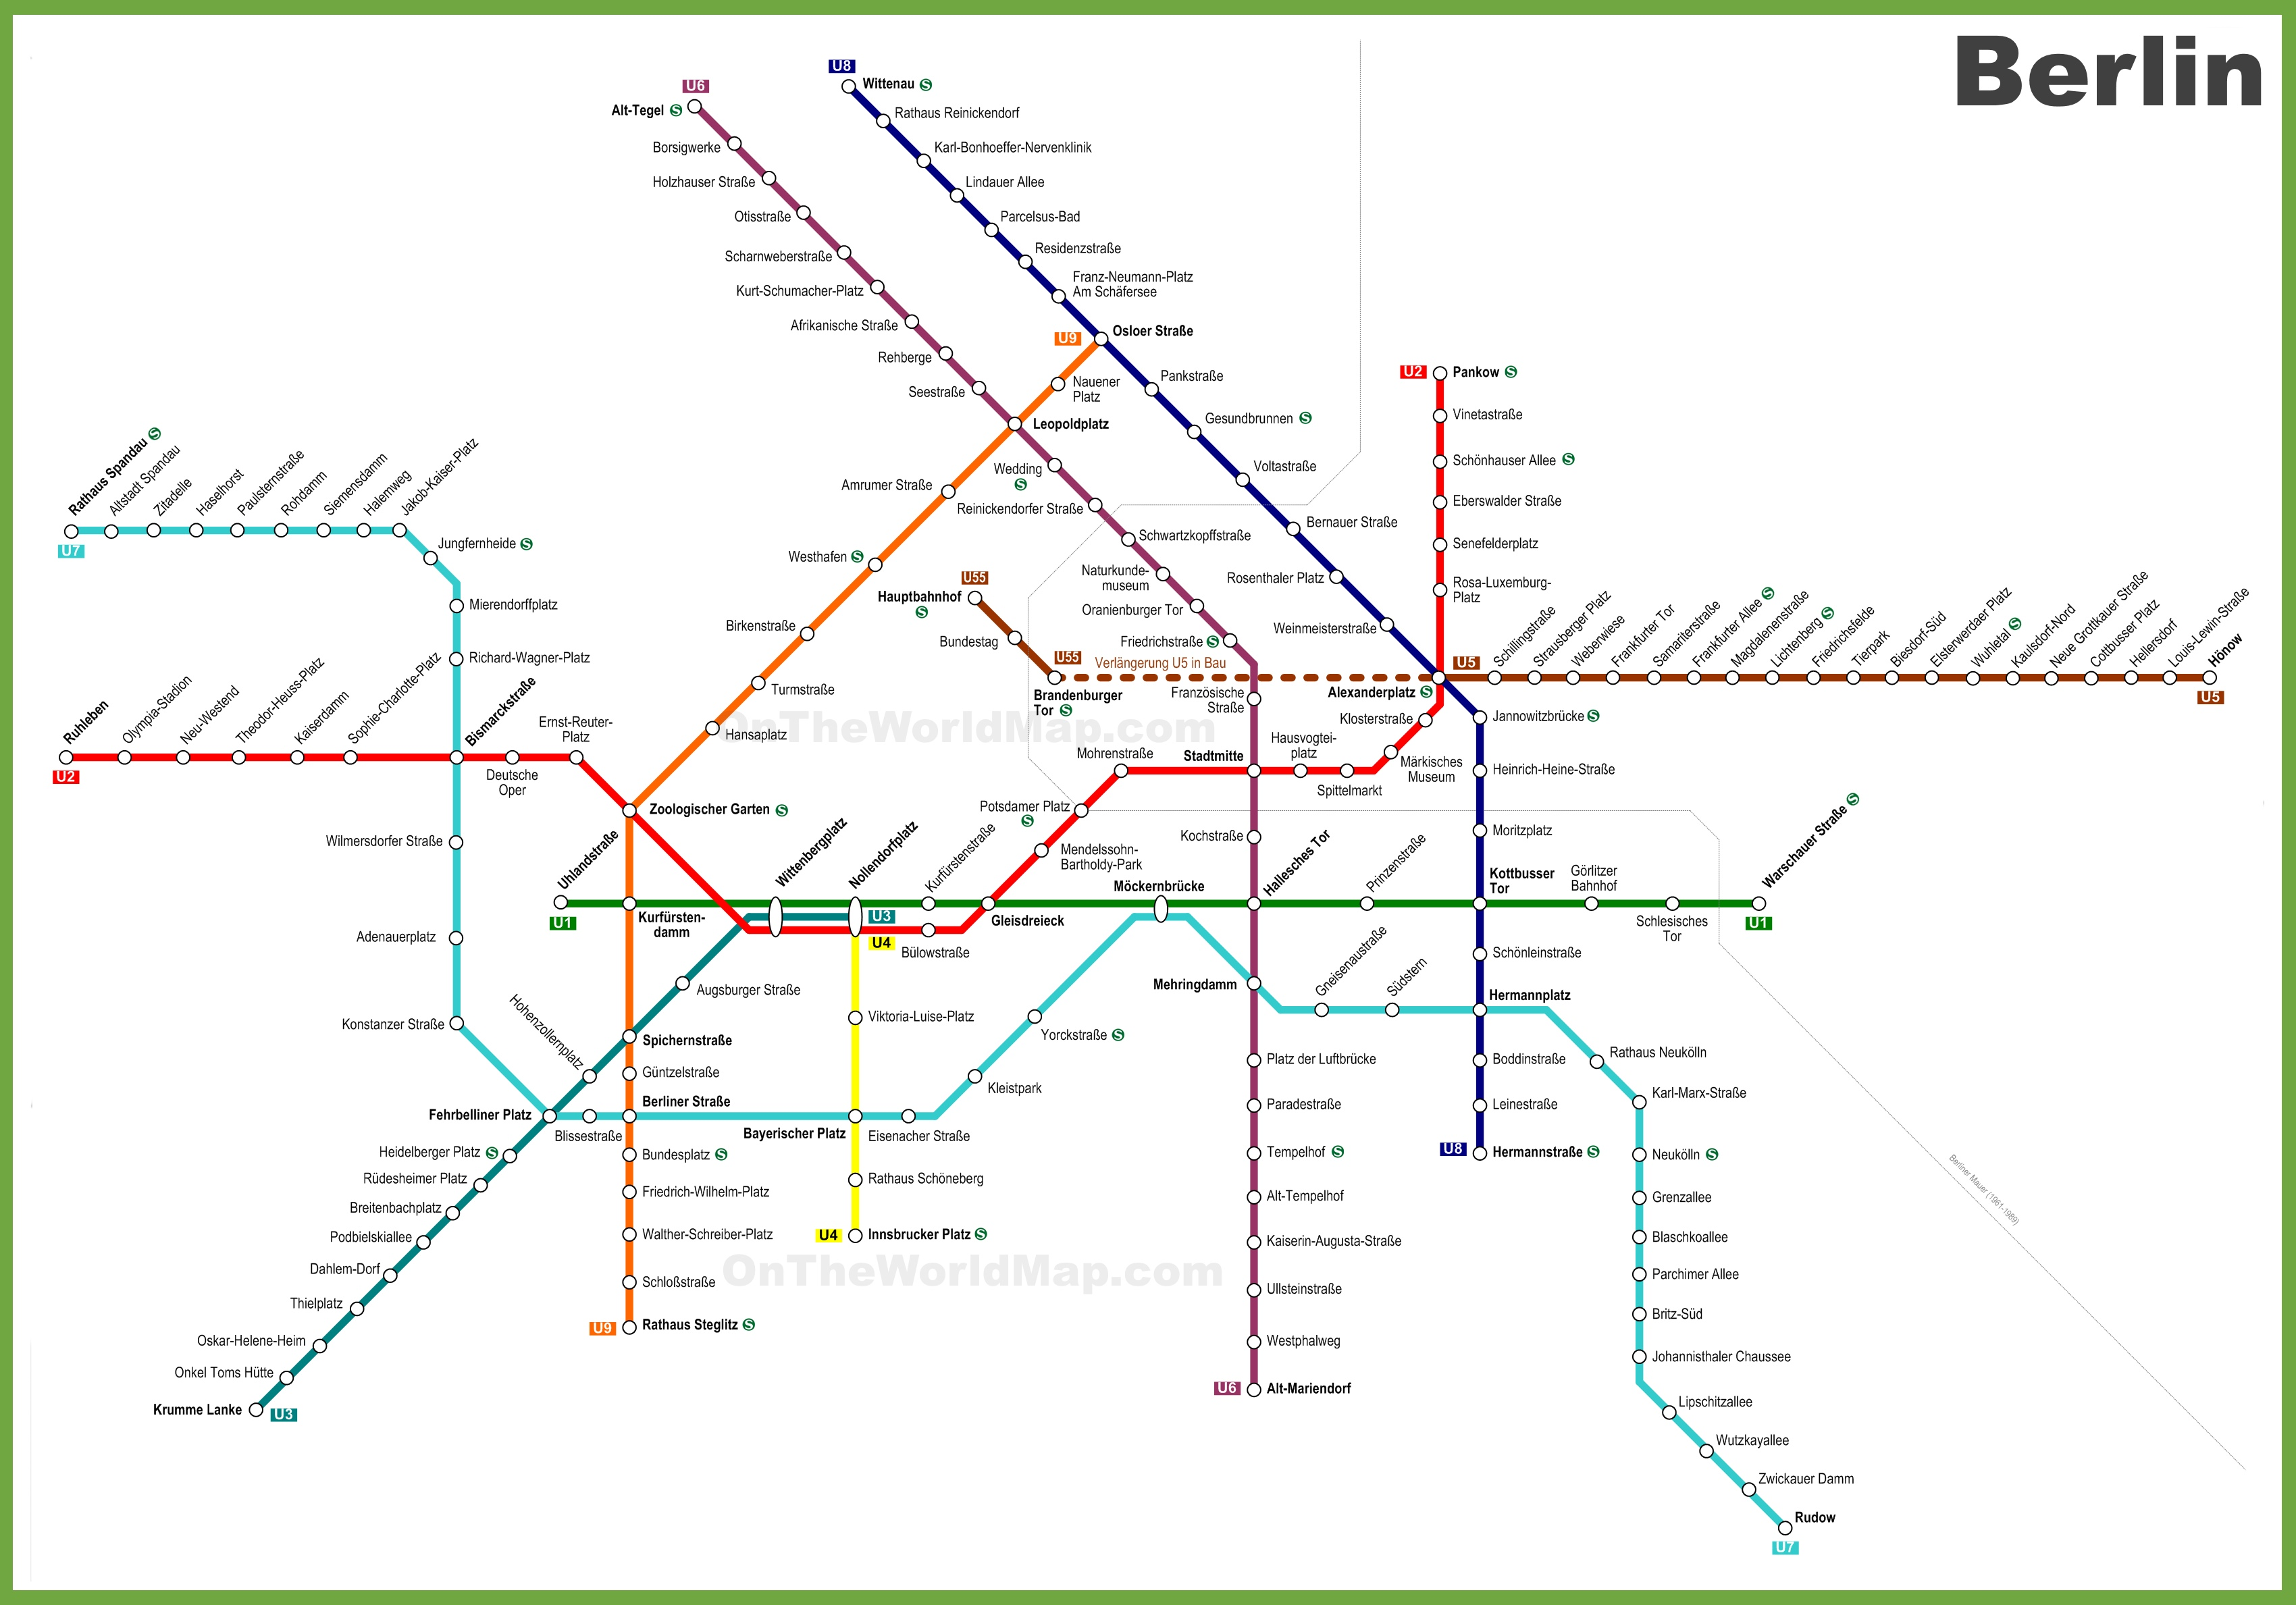
\includegraphics[width=1\textwidth]{images/metro.jpg}}
\caption{\label{legende} Metro de berlin.
}
\end{figure}

\smallbreak

Le métro de Berlin, inauguré en 1902, est composé de 173 station étendu sur 146,3 km. Il est consideré comme un très beau métro.


  \cleardoublepage
  \section{Notice d'utilisation du programme}
\subsection{Compilation}

Ayant dans ma folie fait mon code que dans un seul fichier, la compilation est assez simple. Un simple gcc permet de compiler le fichier. Voici ma commande de compilation :
 \smallbreak

\textit{reset ; gcc -g -W -Wall metro.c && ./a.out}

\subsection{Execution}

A l'execution le programme fourni une liste de station et leurs ID. Puis le programme demande à l'utilisateur d'entré l'ID d'une station puis une autre.
Après peu de temps, le programme fourni un trajet (logiquement le plus cour) a faire pour arriver à destination. Elle est à lire de bas en haut.

\begin{figure}[h]
\centerline{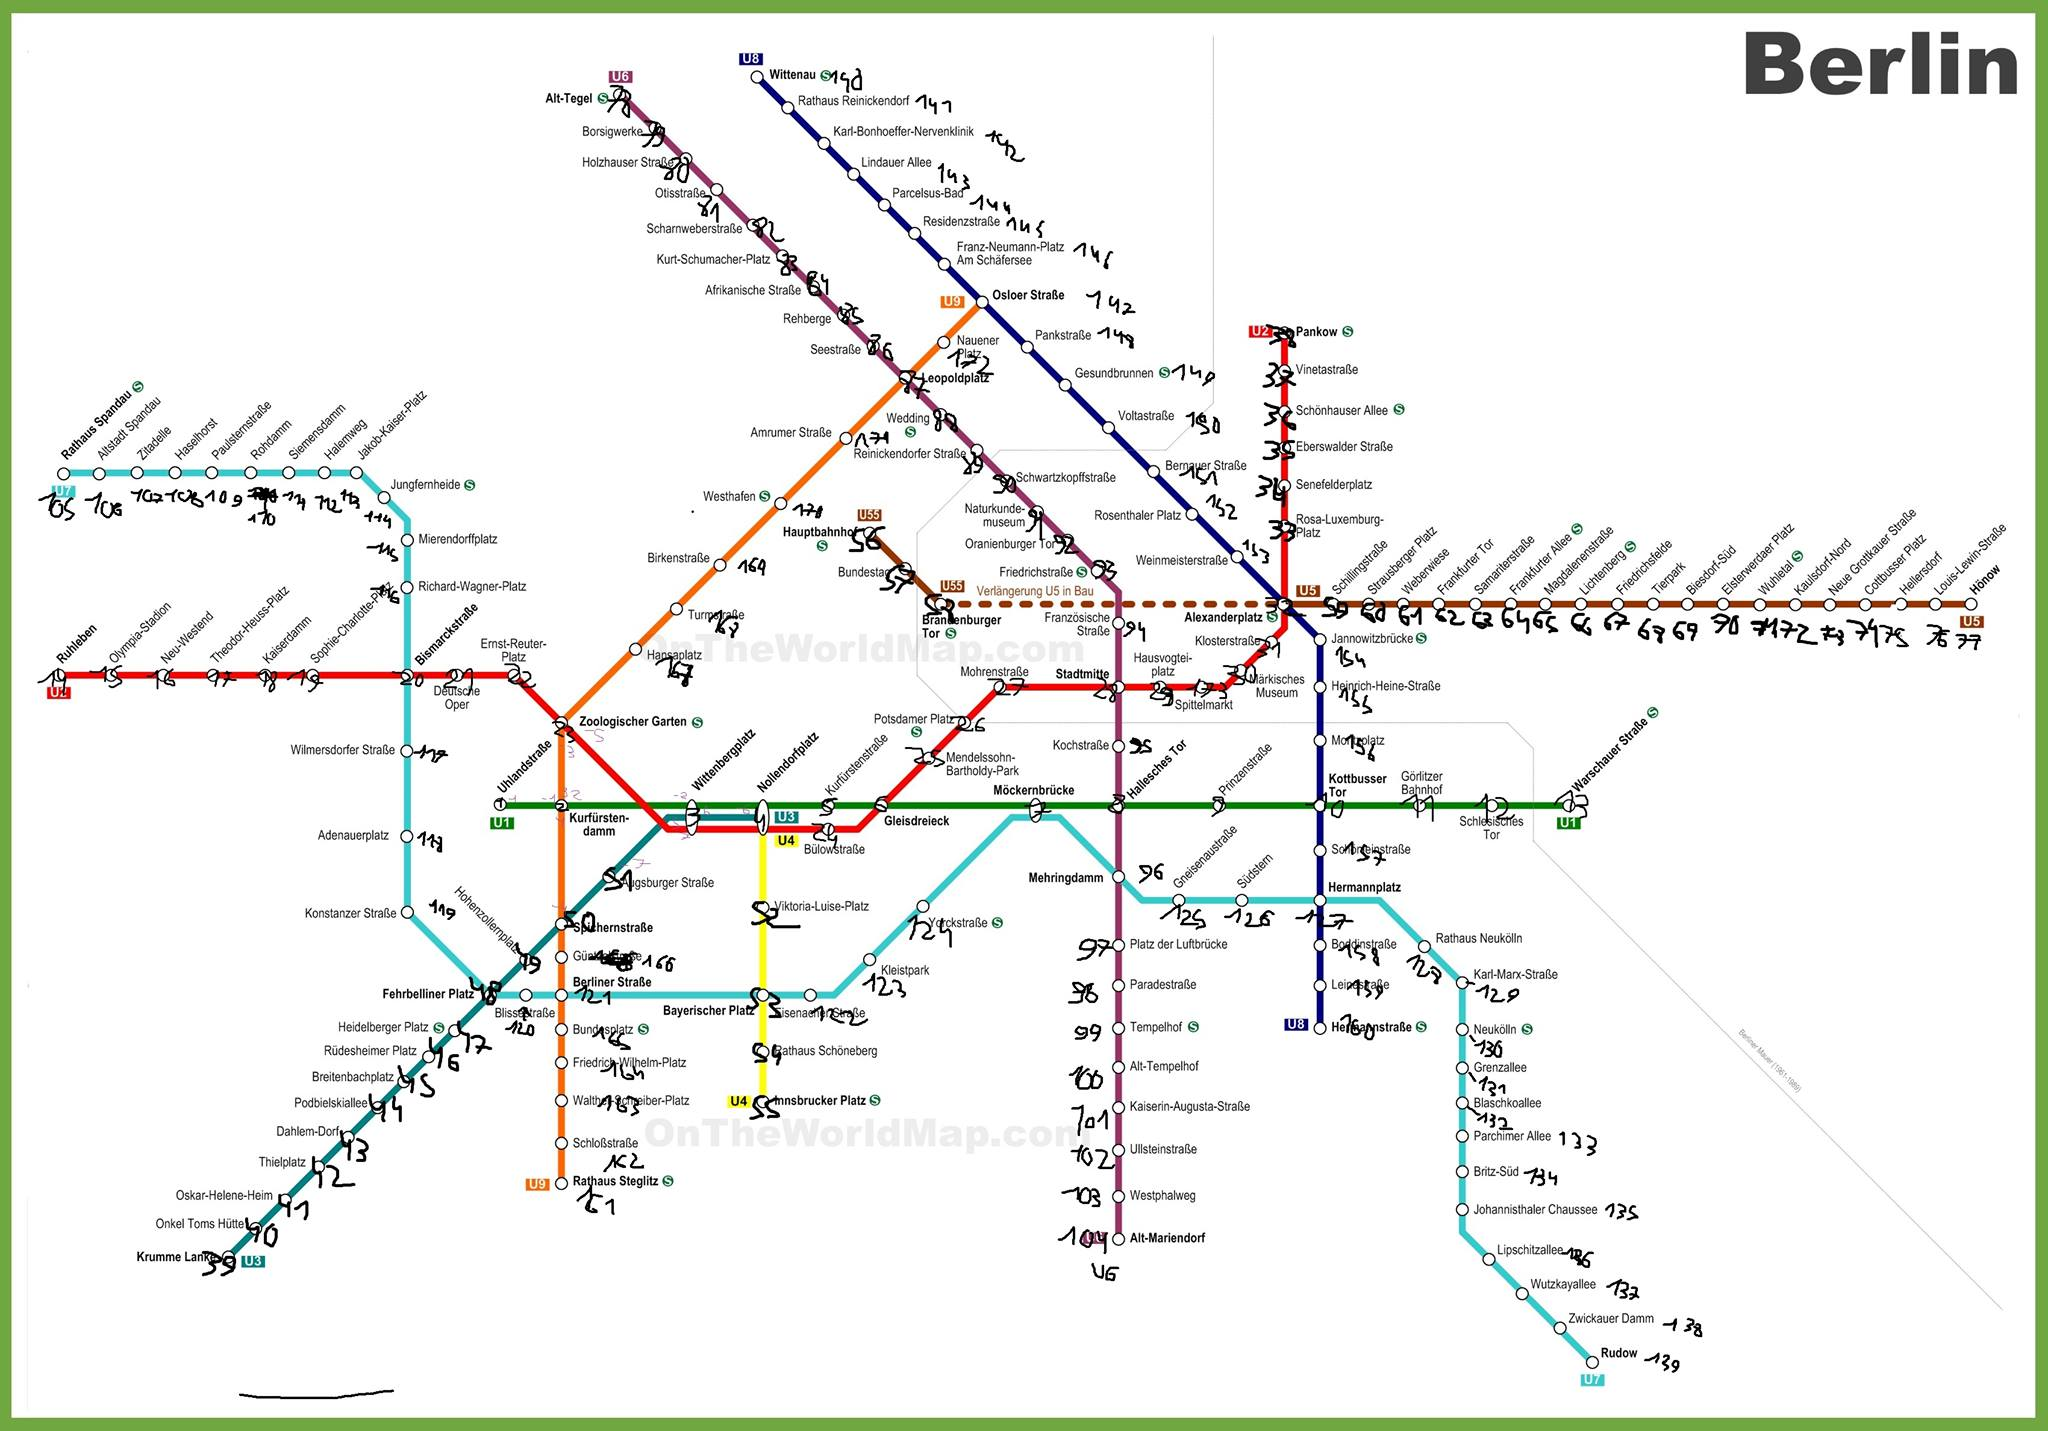
\includegraphics[width=1\textwidth]{images/metroID.jpg}}
\caption{\label{legende} Metro de berlin avec les ID.
}
\end{figure}

  \cleardoublepage
  \section{Explication du code}
\subsection{Les graphes}

Avant de faire l'algorithme, il faut faire son graphe. Et quoi de plus intelligent et beau que de faire son graphe brut et dur dans son code. C'est ainsi que j'ai perdu plusieurs jour à remplir à la main mon graphe en structure vecteur de 2000 lignes station par station correspondance par correspondance. C'est aussi la raison pour laquelle mon programme ne se limite qu'au metro de berlin et ne possede pas en plus les trains/Bus/tramway.
\smallbreak
En ce qui concerne la structure du graphe en brin. N'ayant pas l'idée de refaire la même erreur, j'ai pris les donné du premier graphe et je l'ai est inseré dans le graphes en brin.

\subsection{L'algorithme}
J'utilise une autre structure pour faire fonctionner Djikstra compatible avec les deux version du graphe. C'est une liste de cette structure multiplié par le nombre de station. Elle possède le poid actuel qu'il a fallu pour arriver a la station, la ligne actuel, la station par lequelle elle est arrivé et si l'algorithme est déja passé par cette station.
On initiale cette liste par des valeurs par defaut.
\smallbreak
L'algorithme commence avec trois paramètre en entré : le graphe, l'ID de la station de depart, l'ID de la station d'arrivé. Le code fait bouclé ensuite les stations jusqu'a ce que le second paramètre soit vue.
\smallbreak
Une première boucle verifie que la station n'a pas déja été vue, puis parcours toute les correspondances de la station actuel en ajustant le poid. Si il s'agit de la structure en vecteurs, il parcours les correspondance jusqu'à avoir ateint le nombre de correspondance max, si il s'agit des brins, il parcours tout les brins et brins opposé jusqu'a retombé sur le premier brin de la station d'origine. C'est la seul grosse différence entre les deux algorithmes.
Il complete le le poid de la liste et les autres paramètre. Le code va ensuite choisir de refaire boucler l'algorithme avec la station dont le poids dans la liste est le plus petits. jusqu'a arriver a la station d'arrivé.
Si la station suivante est sur la ligne, le poid est de +1, autrement il est de +2. Le poid est fait en fonction des correspondance et non sur la durée ou la distance. (Bien sur si il y avait un ligne equivalent a la ligne 13, le poid aurait été de +5)
A la fin, le code cite le trajets dans l'ordre inverse. Il faut donc lire le trajets de bas en haut.
Au cas ou, il y a une sécurité pour evité que le programme boucle a l'infini. Je trouve toujours des petites correspondance mal relié ce qui a tendance a faire des choses improbables et bien souvent a bouclé a l'infini lorsqu'il ne trouve pas de station avec un poids inferieur et non vu.

\subsection{Les autres fonctions}
D'autres fonctions plus ou moins utile sont présente. Notamment le main qui semble étrangement être utile. Mais on peut aussi trouver d'autres fonction comme une fonction pour afficher les stations, une autre pour recuperer les entrée saisie des utilisateurs. 4 fonctions pour comparer et recuperer les lignes communes, une fonction pour renvoyer le brin opposé en entré.


  \cleardoublepage
  \section{Le code et moi}
\subsection{Les difficultés}
Dans ce projet, j'ai exprimé beaucoup de difficulté dans beaucoup de domaine. Mes plus grosse furent de comprendre les brins et d'adaptés le précédent graphes en brins (Pour moi les brins sont encore moins intuitifs que les regex). J'ai perdu beaucoup de temps en oubliant a chaque fois que le vecteurs des brins partait de 0  et non pas de -quelquechose, réalisé le graphes fut aussi dur pour moi. J'ai mis beaucoup de temps avant de trouver un moyen de le remplir. En ce qui concerne Dijkstra, l'algorithme en soit n'est pas très compliqué et ne néccessite pas beaucoup de connaissances en mathématiques pour le comprendre mais cette fois ci ce sont beaucoup d'erreurs d'étourderie qui mon fait perdre beaucoup de temps et d'espoirs. 

\subsection{Les améliorations possibles}
Il existe beaucoup beaucouo d'améliorations possible dans mon code. La première serait de creer le graphes autrement qu'en brut nottament avec un fichier texte ou une base de donnée déja disponible sur les data de googles. La secondes (plus esthétique) serait de divisé le programme en plusieurs fichier. Au niveau code, le plus important serait d'améliorer le choix des lignes communes, en effets, mon programme ne se contente que de prendre la premières ligne communes entre les deux stations et ne compare pas la meilleur à prendre. Au niveau optimisation, il y a moyen d'améliorer les ressources en mémoire et temps à utiliser. Nottament en évitant d'appeller plusieurs fois les mêmes fonctions et en stockant les résultat ou encore en changeant les petites valeurs de certaines variables par des char.


  \cleardoublepage
  \section{Conclusion}

Quelque part je ne regrette pas d'avoir pris ce projet.
En plus d'avoir permis de rentabiliser le tutorat de la fac surtout avec une camarades, cela m'as permis d'améliorer ma compréhension des graphes. J'ai aussi grâce a ce projet apris à utilisé GDB ce qui m'aidera par la suites. J'ai aussi appris une leçon, faire une fonction pour remplir un graphes est beaucoup plus rapide que de le faire soit même. J'ai aussi pus decouvrir un peu plus Berlin et je sais maintenant que je ne veux pas y aller même si je ne me perdrais pas dans le métro. Les noms sont bien trop traumatisants pour moi.
  \cleardoublepage
  \section{Code}
\begin{verbatim}
#include "stdio.h"
#include "stdlib.h"
#include "string.h"
#include "assert.h"
#include "limits.h"
#include "time.h"

// Pense Bete : Partir de id-1

typedef struct station {
	int id;
	char nomStation[50];
	char ligne[15];
	struct station ** correspondance;
	int nbCorrespondance;
} station;

typedef struct metro
{
	station * stations;
	int nbstations;
} metro;

typedef struct dijk {
	char dejaVu;
	char ligneActuel;
	int stationAvant;
	int poids;
} dijk;


typedef struct entre{
	int a;
	int b;
} entre;

typedef struct Bstation{
	char nomStation[50];
	char ligne[15];
	int premierBrin;
} Bstation;

typedef struct brin{
	int indexStation;
	int brinSuivant;
} brin;

typedef struct Bmetro {
	Bstation * Bstations;
	int nbStations;
	brin * brins;
	int nbBrins;
} Bmetro;

metro creerMetro(){
	int a = 1;

	// Declaration metro
	metro metroBerlin;
	metroBerlin.nbstations = 173;
	metroBerlin.stations = malloc(sizeof(station)*173);
	assert(metroBerlin.stations);

	// Declaration Station

	station *station1 = metroBerlin.stations;
	station1->id = 1;
	strcpy(station1->nomStation, "Uhlandstraße");
	strcpy(station1->ligne, "U1");
	station1->nbCorrespondance=1;
	station1->correspondance = malloc(sizeof(station*)*station1->nbCorrespondance);
	assert(station1->correspondance);

	station *station2 = metroBerlin.stations+a;
	station2->id = 2;
	strcpy(station2->nomStation, "Kurfürsten-damm");
	strcpy(station2->ligne, "U1 U9");
	station2->nbCorrespondance=4;
	a++;
	station2->correspondance = malloc(sizeof(station*)*station2->nbCorrespondance);
	assert(station2->correspondance);

	station *station3 = metroBerlin.stations+a;
	station3->id = 3;
	strcpy(station3->nomStation, "Wittenberplatz");
	strcpy(station3->ligne, "U1 U2 U3");
	station3->nbCorrespondance=4;
	a++;
	station3->correspondance = malloc(sizeof(station*)*station3->nbCorrespondance);
	assert(station3->correspondance);

	
	[...]


	station *station173 = metroBerlin.stations+a;
	station173->id = 173;
	strcpy(station173->nomStation, "Spittelmarkt");
	strcpy(station173->ligne, "U2");
	station173->nbCorrespondance=2;
	a++;
	station173->correspondance = malloc(sizeof(station*)*station173->nbCorrespondance);
	assert(station173->correspondance);



	// Correspondance Ligne 1

	*(station1->correspondance) = station2;

	*(station2->correspondance) = station1;
	*(station2->correspondance+1) = station3;
	*(station2->correspondance+2) = station23;
	*(station2->correspondance+3) = station50;

	*(station3->correspondance) = station23;
	*(station3->correspondance+1) = station4;
	*(station3->correspondance+2) = station2;
	*(station3->correspondance+3) = station51;

	[...]

	*(station172->correspondance) = station87;
	*(station172->correspondance+1) = station147;
	return metroBerlin;
}


Bmetro creerMetroBrin(metro m){
	int i=0;
	int j=0;
	int b;
	int c;
	//int occ;
	int temp=INT_MAX;
	int temp2=INT_MAX;
	//maloc du nombre de correspondance*2+1 pour l'index 0 ?
	//Declaration metro
	Bmetro BmetroBerlin;
	BmetroBerlin.nbStations = m.nbstations;
	BmetroBerlin.Bstations = malloc(sizeof(Bstation)*(BmetroBerlin.nbStations));
	BmetroBerlin.nbBrins = 1;
	for(i=0; i<m.nbstations; i++){
		BmetroBerlin.nbBrins+=((m.stations+i)->nbCorrespondance);
	}
	BmetroBerlin.brins = malloc(sizeof(Bstation)*BmetroBerlin.nbBrins);
	assert(BmetroBerlin.Bstations);
	for(i=0; i<m.nbstations;i++){
		strcpy((BmetroBerlin.Bstations+i)->nomStation, (m.stations+i)->nomStation);
		strcpy((BmetroBerlin.Bstations+i)->ligne, (m.stations+i)->ligne);
	}
	
	//Initialisation Brin
	for(i=0; i<BmetroBerlin.nbBrins;i++){
		(BmetroBerlin.brins+i)->brinSuivant=INT_MAX;
		(BmetroBerlin.brins+i)->indexStation=INT_MAX;
	}
	for(i=0; i<BmetroBerlin.nbStations;i++){
		(BmetroBerlin.Bstations+i)->premierBrin=INT_MAX;
	}
	b=1;
	for(i=0; i<BmetroBerlin.nbStations;i++){
		for(j=0; j<(m.stations+i)->nbCorrespondance; j++){
			c=(*((m.stations+i)->correspondance+j))->id-1;
			if(i < c){
				if((BmetroBerlin.Bstations+c)->premierBrin==INT_MAX)
					(BmetroBerlin.Bstations+c)->premierBrin=BmetroBerlin.nbBrins/2-b;
				if((BmetroBerlin.Bstations+i)->premierBrin==INT_MAX)
					(BmetroBerlin.Bstations+i)->premierBrin=BmetroBerlin.nbBrins/2+b;
				(BmetroBerlin.brins+(BmetroBerlin.nbBrins/2+b))->indexStation=i;
				(BmetroBerlin.brins+(BmetroBerlin.nbBrins/2-b))->indexStation=c;
				b++;
			}
			//printf("%d\n", b);
		}
	}
	// Debug :
	// for(i=0; i<BmetroBerlin.nbBrins; i++){
	// 	if(i > 185)
	// 		printf("Brin %d(%d)-> %d Brin Suivant :\n", i, i-BmetroBerlin.nbBrins/2,(BmetroBerlin.brins+i)->indexStation);
	// 	if(i == 185)
	// 		printf("Brin %d(0) -> %d Brin Suivant :\n", i, (BmetroBerlin.brins+i)->indexStation);
	// 	if(i < 185)
	// 		printf("Brin %d(%d)-> %d Brin Suivant :\n", i, i-(BmetroBerlin.nbBrins/2),(BmetroBerlin.brins+i)->indexStation);
	// }
	for(i=0; i<BmetroBerlin.nbStations; i++){
			for(j=0;j<BmetroBerlin.nbBrins; j++){
				//printf("%d\n", j);
				if((BmetroBerlin.brins+j)->indexStation == i){
					temp = j;
					temp2 = j;
					(BmetroBerlin.brins+j)->brinSuivant = temp;
					j++;
					break;
				}
			}
			while(j<BmetroBerlin.nbBrins){
				if((BmetroBerlin.brins+j)->indexStation == i){
					(BmetroBerlin.brins+j)->brinSuivant = temp2;
					temp2 = j;
				}
				j++;
			}
			(BmetroBerlin.brins+temp)->brinSuivant =temp2;
	}
	printf("\n\n\n");

	// debug
	// for(i=0; i<BmetroBerlin.nbBrins; i++){
	// 	if(i > 185)
	// 		printf("Brin %d(%d)-> %d Brin Suivant :%d\n", i, i-BmetroBerlin.nbBrins/2,(BmetroBerlin.brins+i)->indexStation, (BmetroBerlin.brins+i)->brinSuivant);
	// 	if(i == 185)
	// 		printf("Brin %d(0) -> %d Brin Suivant :%d\n", i, (BmetroBerlin.brins+i)->indexStation, (BmetroBerlin.brins+i)->brinSuivant);
	// 	if(i < 185)
	// 		printf("Brin %d(%d)-> %d Brin Suivant : %d\n", i, i-(BmetroBerlin.nbBrins/2),(BmetroBerlin.brins+i)->indexStation, (BmetroBerlin.brins+i)->brinSuivant);
	// }
	return BmetroBerlin;
}


void afficheStation(metro m){
	int i;
	for(i=0; i < m.nbstations; i++){
		printf("La station %d se nomme : \033[4m%s\033[0m disponible sur la/les ligne(s) : %s.\n",i+1,(m.stations+i)->nomStation, (m.stations+i)->ligne);
	}
}

void afficheStation2(Bmetro m){
	int i;
	for(i=0; i < m.nbStations; i++){
		printf("La station %d se nomme : \033[4m%s\033[0m disponible sur la/les ligne(s) : %s.\n",i+1,(m.Bstations+i)->nomStation, (m.Bstations+i)->ligne);
	}
}

char memeLigne2(metro m, char ligneActuel, int idb){
	int i;

	for(i=1; i < 11;i=i+3){
		//printf("%c =? %c\n", temp1[i], temp2[j]);
		if((m.stations+idb)->ligne[i] == ligneActuel && (m.stations+idb)->ligne[i-1] == 'U')
			return 1;
	}
	return 0;
}

char BmemeLigne(Bmetro m, char ligneActuel, int idb){
	int i;

	for(i=1; i < 11;i=i+3){
		//printf("%c =? %c\n", temp1[i], temp2[j]);
		if((m.Bstations+idb)->ligne[i] == ligneActuel && (m.Bstations+idb)->ligne[i-1] == 'U')
			return 1;
	}
	return 0;
}

char ligneComp(metro m, int ida, int idb){
	//printf("Appel ligneComp\n");
	int i;
	int j;

	for(j=1; j < 11;j=j+3){
		for(i=1; i < 11;i=i+3){
			if((m.stations+ida)->ligne[i] == (m.stations+idb)->ligne[j]){
				//printf("Insertion boucle avec : %c\n", (m.stations+ida)->ligne[i]);
				return (m.stations+ida)->ligne[i];
			}
		}
	}
	return 0;
}

char BligneComp(Bmetro m, int ida, int idb){
	//printf("Appel ligneComp\n");
	int i;
	int j;

	for(j=1; j < 11;j=j+3){
		for(i=1; i < 11;i=i+3){
			if((m.Bstations+ida)->ligne[i] == (m.Bstations+idb)->ligne[j]){
				//printf("Insertion boucle avec : %c\n", (m.stations+ida)->ligne[i]);
				return (m.Bstations+ida)->ligne[i];
			}
		}
	}
	return 0;
}

int oppose(Bmetro m, int brin){
	int temp = brin;
	if(brin < m.nbBrins){
		temp = (m.nbBrins/2)-brin;
		brin = (m.nbBrins/2)+temp;
		return brin;
	}
	else{
		brin = (m.nbBrins)-brin;
		return brin;
	}

}

void dijkstraPurSansModificationJulie(metro m, int ida, int idb){
	int securite;
	int i;
	int b;
	int debut = ida;
	int poids;
	dijk liste[m.nbstations];

	// Initiation Dijkstra
	for(i=0;i<m.nbstations;i++){
		liste[i].dejaVu = 0;
		liste[i].poids = INT_MAX;
		liste[i].stationAvant = -1;
	}
	liste[ida].poids = 0;
	liste[ida].ligneActuel = 0;

	//Dijkstra
	while(ida != idb){
		liste[ida].dejaVu = 1;
		
		// Traitement des correspondances.
		for(i=0; i < (m.stations+ida)->nbCorrespondance; i++){
			b= ((*((m.stations+ida)->correspondance+i))->id-1);
			if(liste[b].dejaVu !=1){
				// Erreur Potentiel, id-1 pour l'index 0 ? Trop de confusion. Note a moi même : faire le fucking début de graphes a 0 pour eviter la confusion.
				if(memeLigne2(m, liste[ida].ligneActuel, b)){
					poids = liste[ida].poids+1;
				}
				else{
					poids = liste[ida].poids+2;
				}
				if(poids < liste[b].poids){
					if(memeLigne2(m, liste[ida].ligneActuel, b))
						liste[b].ligneActuel = liste[ida].ligneActuel;
					else
						liste[b].ligneActuel = ligneComp(m, ida, b);
					liste[b].poids = poids;
					liste[b].stationAvant = (m.stations+ida)->id-1;
				}
			}
		}
		securite = ida;
		poids = INT_MAX;
		for(i=0; i<m.nbstations;i++){

			if(!liste[i].dejaVu && liste[i].poids<poids){
				poids = liste[i].poids;
				ida = i;
			}
		}	
		if(ida == securite){
			printf("%d\n", ida);
			printf("La station %s n'as pas pus être atteinte, allez y à pied.\n", (m.stations+idb)->nomStation);
			return;
		}
	}
	// Affichage de bas en haut
	i = idb;
	printf("Attention, Le trajet se lit de bas en haut !\n\n");
	while(i!=debut){
		printf("%s via la ligne U%c\n", (m.stations+i)->nomStation, liste[i].ligneActuel);
		i = liste[i].stationAvant;
	}
	printf("%s\n", (m.stations+debut)->nomStation);
}


void DijkstraBrin(Bmetro m, int ida, int idb){
	int securite;
	int i;
	int b;
	int debut = ida;
	int poids;
	int temp;
	int c;
	int temp2;
	int brinop;
	dijk liste[m.nbStations];

	// Initiation Dijkstra
	for(i=0;i<m.nbStations;i++){
		liste[i].dejaVu = 0;
		liste[i].poids = INT_MAX;
		liste[i].stationAvant = -1;
	}
	liste[ida].poids = 0;
	liste[ida].ligneActuel = 0;

	//Dijkstra
	while(ida != idb){
		liste[ida].dejaVu = 1;
		temp = INT_MAX;
		c = 0;

		temp2 = (m.brins+((m.Bstations+ida)->premierBrin))->brinSuivant;
		brinop = oppose(m, (m.Bstations+ida)->premierBrin);
		b = (m.brins+brinop)->indexStation;
		while(temp != (m.Bstations+ida)->premierBrin){
			if(c){
					brinop = oppose(m, temp);
					b = (m.brins+brinop)->indexStation;
			}else{

				c++;
			}
			temp = temp2;
			temp2 = (m.brins+temp)->brinSuivant;
			if(liste[b].dejaVu != 1){
				if(BmemeLigne(m, liste[ida].ligneActuel, b))
					poids = liste[ida].poids+1;
			}
			else{
				poids = liste[ida].poids+2;
			}
			if(poids < liste[b].poids){
				if(BmemeLigne(m, liste[ida].ligneActuel, b))
						liste[b].ligneActuel = liste[ida].ligneActuel;
				else
					liste[b].ligneActuel = BligneComp(m, ida, b);
				liste[b].poids = poids;
				liste[b].stationAvant = ida;
			}
		}
		securite = ida;
		poids = INT_MAX;
		for(i=0; i<m.nbStations;i++){

			if(!liste[i].dejaVu && liste[i].poids<poids){
				poids = liste[i].poids;
				ida = i;
			}
		}	
		if(ida == securite){
			printf("%d\n", ida);
			printf("La station %s n'as pas pus être atteinte, allez y à pied.\n", (m.Bstations+idb)->nomStation);
			return;
		}
	}
	// Affiche de bas en haut
	printf("Attention, Le trajet se lit de bas en haut !\n\n");
	i = idb;
	while(i!=debut){
		printf("%s via la ligne U%c\n", (m.Bstations+i)->nomStation, liste[i].ligneActuel);
		i = liste[i].stationAvant;
	}
	printf("%s\n", (m.Bstations+debut)->nomStation);
}


entre recupStation(){
	entre ut;
	ut.a = 0;
	ut.b = 0;
		printf("Entrer la station de départ :\n");
		scanf("%d", &ut.a);

		printf("Entrer la station d'arrivé :\n");
		scanf("%d", &ut.b);
	return ut;
}

int main(){
	clock_t debut;
	debut = clock();
	metro metroBerlin = creerMetro();
	Bmetro BmetroBerlin = creerMetroBrin(metroBerlin);
	printf("\nTemps : %f\n", (double)(clock () - debut) / CLOCKS_PER_SEC);
	afficheStation(metroBerlin);
	entre ut = recupStation();
	//afficheStation2(BmetroBerlin);
	debut = clock();
	printf("\n\nStructure Vecteur :\n\n");
	dijkstraPurSansModificationJulie(metroBerlin, (ut.a-1), (ut.b-1));
	printf("\n\nStructure Brin :\n\n");
	DijkstraBrin(BmetroBerlin, (ut.a-1), (ut.b-1));
	printf("\nTemps : %f\n", (double)(clock () - debut) / CLOCKS_PER_SEC);
}

\end{verbatim}

\end{document}

